%===============================================================================
%===============================================================================
%
\subsection{Example-0001}
%
%===============================================================================
%
\subsubsection{Model}
%
We solve the following equation,
%
\begin{align}
    \nabla \cdot \nabla u = 0 & &&\Omega \in [0, 2] \times [0, 1] \times [0, 1],
\end{align}
%
with boundary conditions
%
\begin{align}
    u = 0 & &&x = y = z = 0, \\
    u = 0 & &&x = 2, y = z = 1.
\end{align}
%
No material parameters to specify.
%
%===============================================================================
%
\subsubsection{Results}
%
\begin{figure}[h!]
    \centering 
    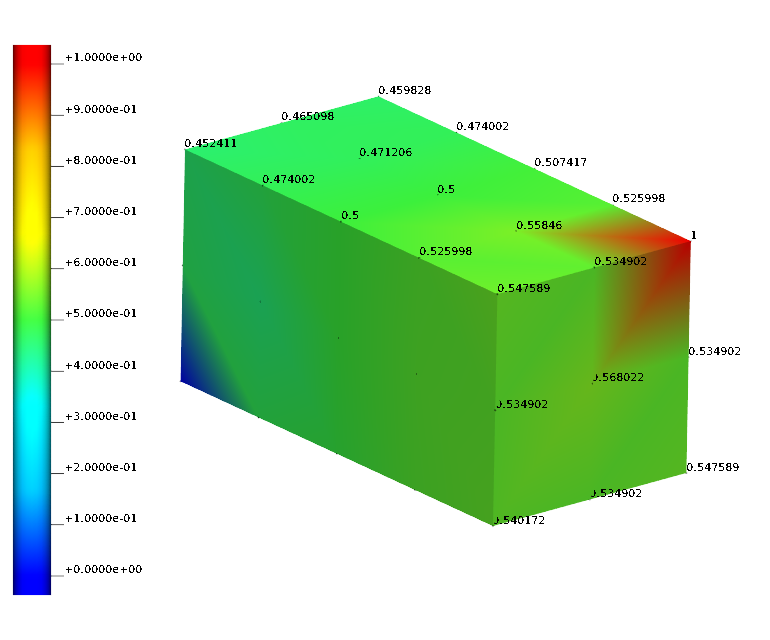
\includegraphics[width=\columnwidth]{examples/example-0001/figures/example.png} 
    \caption{Results.}
    \label{example-0001-fig}
\end{figure}
%
%===============================================================================
%===============================================================================
